\subsection{Chirowaveguides considered in \cite{wujaggard}}
In \cite{wujaggard}, the authors consider a metallic waveguide 
which is air filled except for an obstacle
characterized by a chiral media  with the following constitutive relations. 

\begin{equation}
\left\{
\begin{array}{ll}
{\bf D} = \varepsilon_0\varepsilon_r I_3 {\bf E} - j \xi_c I_3 {\bf B} \\
{\bf H} = -j\xi_c I_3 {\bf E} + \frac{1}{\mu_0\mu_r} I_3 {\bf B}.
\end{array}
\right.
\end{equation}

Here $\varepsilon_r$, $\mu_r$ and $\xi_c$ are strictly positive real quantities.
Thus from \eqref{eq:constitutiveeqn} we easily can easily identify $P$, $Q$, $L$
and $M$ which are given below.

\begin{equation} \label{constitutive_wu_P}
P = \varepsilon_0\varepsilon_rc_0 I_3 
\end{equation}

\begin{equation} \label{constitutive_wu_Q}
Q = \frac{1}{\mu_0\mu_rc_0} I_3
\end{equation}

\begin{equation} \label{constitutive_wu_LM}
L = M = -j\xi_cI_3
\end{equation}

In \cite{bianisotropi_m3as} it was shown that this media could not be managed by the previous theory
developed there.
However, the generality of the present theory allows us to apply it to obtain 
the conditions for well-posedness and finite element approximability of this kind 
of problem of practical interest.

Here we analyze the validity of the hypotheses by considering $\varepsilon_r > 1$ 
and $\mu_r =1$.
$P_s$ is equal to $\varepsilon_0 \varepsilon_r c_0$ inside material 
and simply $\varepsilon_0 c_0$ outside.
Since $\Omega_{el} = \emptyset$,  $C_{PS}$ is equal to $C_2$ defined in 
\eqref{eq:c2_constant} and has a value $\varepsilon_0 c_0$, 
verifying the hypothesis H5.
The hypothesis H6 is also trivially valid and $C_{QS} = \frac{1}{\mu_0 c_0}$. 
By equations \eqref{equation_for_CL} and \eqref{equation_for_CM}, $C_L = C_M =  |\xi_c|$.
Then the inequality in hypothesis H7 becomes  
$C_{QS} - \frac{C_L C_M}{C_{PS}} = \frac{1}{c_0}(\frac{1}{\mu_0} - \frac{\xi_c^2}{\varepsilon_0}) > 0$ 
which implies

\begin{equation} \label{eq:inf_sup_wu_jaggard}
\xi_c < \sqrt{\frac{\varepsilon_0}{\mu_0}} = 2.654 \, 10^{-3}  \text{ mho }.
\end{equation}

This is not a small value considering the chiral effects reported in \cite{wujaggard}. 
Now we need to verify the hypotheses H1-H4 which need to hold true locally and hence
we have to examine only media inside the obstacle which is bianisotropic. 
For doing this the suitable form 
of constitutive relations is in terms of $\kappa$, $\nu$, $\gamma$ and $\chi$ 
which are given by the following \cite{noiregolarita}. 

\begin{equation}
\kappa = \frac{1}{\varepsilon_0\varepsilon_r}I_3
\end{equation}

\begin{equation}
\nu = \frac{\varepsilon_0\varepsilon_r+\mu_0\xi_c^2}{\mu_0\varepsilon_0\varepsilon_r}I_3
\end{equation}

\begin{equation}
\chi = -\gamma = \frac{j\xi_c}{\varepsilon_0\varepsilon_r}I_3
\end{equation}

$\kappa$ and $\nu$ are multiples of the identity matrix with eigenvalues $\varepsilon_0\varepsilon_r$ 
and $(\frac{\varepsilon_0\varepsilon_r+\mu_0\xi_c^2}{\mu_0\varepsilon_0\varepsilon_r})$ respectively.
The determinants are just the cubes of the eigenvalues and hence according to equations 
\eqref{equation_for_C_kd} and \eqref{equation_for_C_nud} we get the values of $C_{\kappa,d}$ and 
$C_{\nu,d}$

\begin{equation}
C_{\kappa,d} = \left(\frac{1}{\varepsilon_0\varepsilon_r}\right)^3
\end{equation}

\begin{equation}
C_{\nu,d} = \left(\frac{\varepsilon_0\varepsilon_r+\mu_0\xi_c^2}{\mu_0\varepsilon_0\varepsilon_r}\right)^3
\end{equation}

$C_{\kappa,s}$ and $C_{\nu,s}$ by equations \eqref{equation_for_C_ks} and \eqref{equation_for_C_nus} 
are in this case simply twice the eigenvalue of corresponding diagonal matrix.

\begin{equation}
C_{\kappa,s} = \frac{2}{\varepsilon_0\varepsilon_r}
\end{equation}

\begin{equation}
C_{\nu,s} = 2\frac{\varepsilon_0\varepsilon_r+\mu_0\xi_c^2}{\mu_0\varepsilon_0\varepsilon_r}
\end{equation}

The inverse of the matrices are also trivial and equations \eqref{equation_for_C_kr} and \eqref{equation_for_C_nur} simply
evaluate to the reciprocals of eigenvalues of $\kappa$ and $\nu$ respectively giving $C_{\kappa,r}$ and $C_{\nu,r}$. 

\begin{equation}
C_{\kappa,r} = \varepsilon_0\varepsilon_r
\end{equation}

\begin{equation}
C_{\nu,r} = \frac{\mu_0\varepsilon_0\varepsilon_r}{\varepsilon_0\varepsilon_r+\mu_0\xi_c^2}
\end{equation}

From equations \eqref{equation_for_C_chis} and \eqref{equation_for_C_gammas} we get

\begin{equation}
C_{\chi,s} = C_{\gamma,s} = \frac{\xi_c}{\varepsilon_0\varepsilon_r}.
\end{equation}

Having shown that the hypotheses H1-H3 are satisfied, we can use the above 
constants to calculate $K_u$ and then to verify H4.
Figure \ref{fi:wu_jaggard_regularity_factor_vs_xi} shows the dependence of 
$K_u$ on $\xi_c$ for various values of $\varepsilon_r$.
As the value of $\varepsilon_r$ increases, the hypothesis H4 remains valid
for higher and higher value of $\xi_c$.
Figure \ref{fi:critical_value_of_xi_for_uniqueness_wu_jaggard} shows the
plot of the critical value of $\xi_c$ below which H4 is satisfied against 
$\varepsilon_r$.
The limit of $2.654 \, 10^{-3}$ arising from equation \eqref{eq:inf_sup_wu_jaggard}
required for satisfying H7 is also shown in the same figure.
It is seen that for low values of $\varepsilon_r$ the tighter condition arises from
the need to satisfy H4.
For example the limiting value is $5.6 \, 10^{-4}$ for $\varepsilon_r=1$ and increases
with $\varepsilon_r$ and is $1.78 \, 10^{-3}$ for $\varepsilon_r = 10$.
The curve crosses  $2.654 \, 10^{-3}$ mho line at around $\varepsilon_r = 22.3$ and 
above that value equation \eqref{eq:inf_sup_wu_jaggard} imposes the stricter limit. 

\begin{figure}
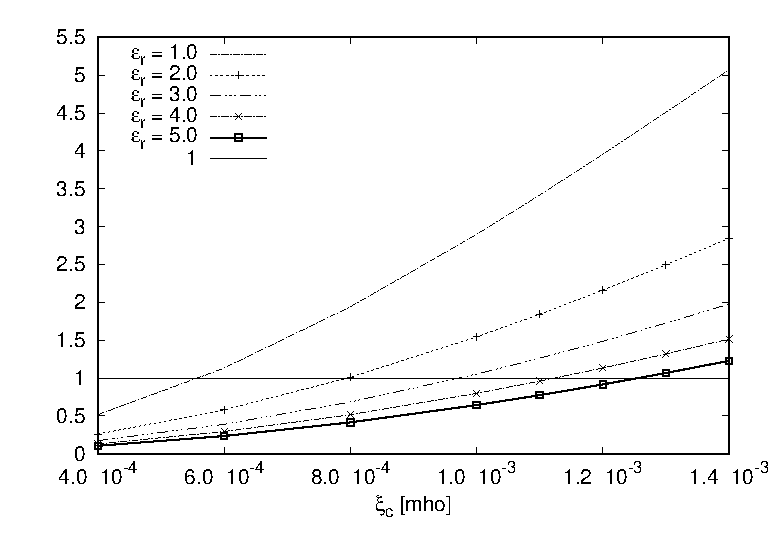
\includegraphics{regularity_factor_vs_xi_wu_jaggard.eps}
\caption{Plot of $K_u$ versus $\xi_c$ for the bianisotropic medium described in \cite{wujaggard}.
The plots are shown for various values of $\varepsilon_r$. 
The hypothesis H4 is satisfied for $K_u < 1$.}
\label{fi:wu_jaggard_regularity_factor_vs_xi}
\end{figure}

\begin{figure}
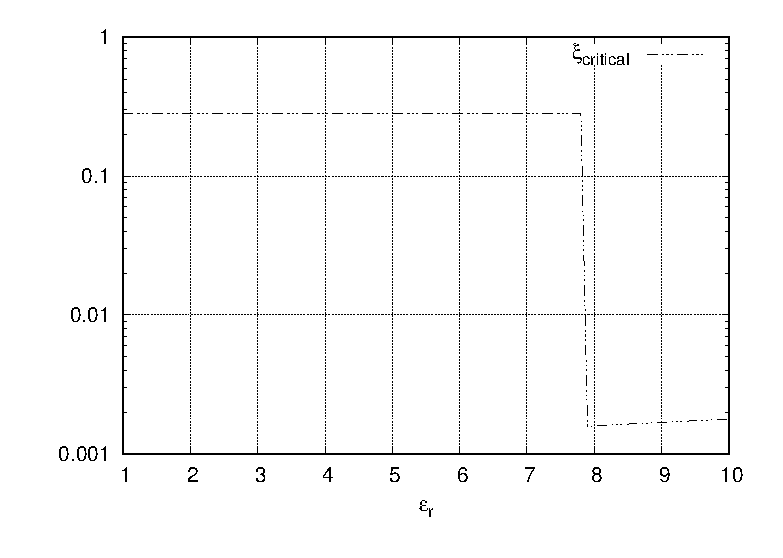
\includegraphics{graphical_analysis_related_to_uniqueness_wu_jaggard.eps}
\caption{The value of $\xi_c$ below which the hypothesis H4
is satisfied is plotted against $\varepsilon_r$.
The limit of $2.654 \, 10^{-3}$ arising from equation \eqref{eq:inf_sup_wu_jaggard}
required for satisfying H7 is also shown.}
\label{fi:critical_value_of_xi_for_uniqueness_wu_jaggard}
\end{figure}

Now we consider a specific numerical problem for which the solution can serve as benchmark 
for other approaches and solvers owing to the reliability of the results guaranteed by the theory.
A rectangular waveguide with a discontinuity due to a block of bianisotropic medium is considered 
as shown in Figure \ref{fi:geometry_wujaggard}.
In the simulation the rectangular waveguide is characterized by  $a=23$ mm, $b=10$ mm  and has a length $l=40$ mm.
The obstacle is a parallelepiped with  $c=11$ mm, $d=5$ mm and length $w=10$ mm.
The origin of the axis is at the lower right corner of the near face of the waveguide shown in Figure \ref{fi:geometry_wujaggard}.
The obstacle ranges from $x = 6$ mm to $x=17$ mm along the x axis, 
from $y=0$ to $y=5$ mm along the y axis and from $z=15$ mm to $z=25$ mm along the z axis.
The bianisotropic medium making up the obstacle is characterized by $\varepsilon_r = 5$ 
and $\xi_c = 1.24\, 10^{-3}$.
For this medium $K_u=0.98 < 1 $ and also equation \eqref{eq:inf_sup_wu_jaggard} is satisfied
and hence all the hypotheses required to guarantee the well posedness and convergence of finite element
solution hold true.
The waveguide is excited with $TE_{10}$ mode with amplitude of 1 $V/m$ and frequency of 9 GHz.

\begin{figure}
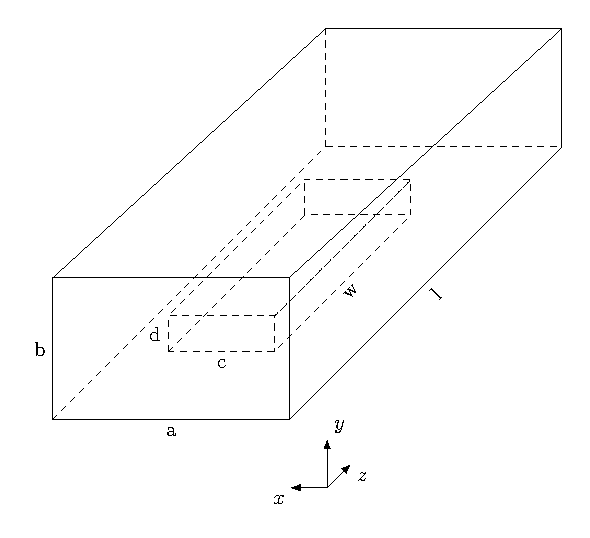
\includegraphics[scale=1.2]{draw_waveguide_wu_jaggard.eps}
\caption{The geometry of a rectangular waveguide partially filled with chiral media considered in \cite{wujaggard}.}
\label{fi:geometry_wujaggard}
\end{figure}

The details of the Galerkin finite element solver is the same as before.
The tetrahedral meshes are also obtained in a similar way as discussed in the previous subsection
by dividing the domain into small cubes each of which are in turn subdivided into six tetrahedra.
The convergence of the solution is verified by checking the solutions for three different meshes
which are characterized by small cubes of sides 0.5 mm, 0.25 mm and 0.167 mm which are references as,
respectively, ``coarse'', ``fine'' and ``very fine'' meshes.
There are 10824 nodes, 55200 elements and 6200 boundary faces in coarse mesh,
where as the fine mesh has 79947 nodes, 441600 elements and 24800 boundary faces and 
finally the very fine mesh has 262570 nodes, 1490400 elements and 55800 boundary faces.
The solutions obtained were very stable which is illustrated by showing the results obtained 
for the x component of the magnitude of the electric field along the y axis with
these meshes in Figure \ref{fi:wu_jaggard_convergence}.

\begin{figure}
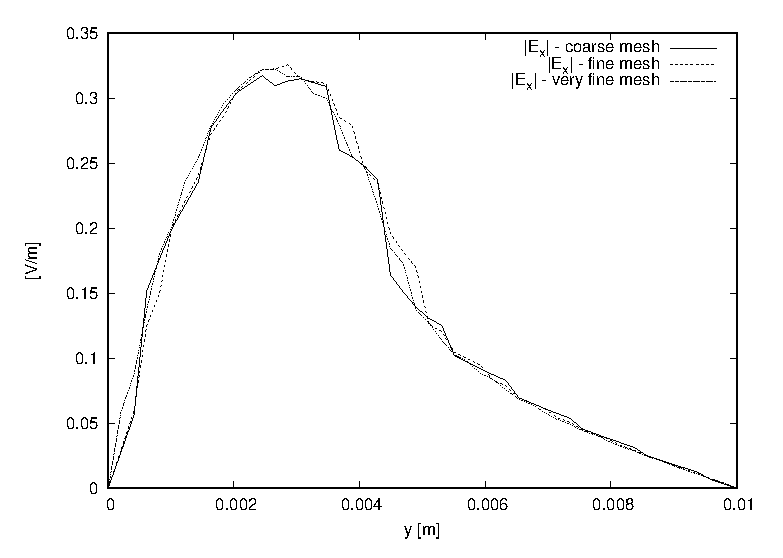
\includegraphics{figure_convergence_wu_jaggard_along_y_mag_ex.eps}
\caption{Convergence of the solution for problem involving medium in \cite{wujaggard}.
The magnitude of the $x$ component of the electric field is plotted 
along a line parallel to $y$ axis for four different meshes.}
\label{fi:wu_jaggard_convergence}
\end{figure}

Figures  \ref{fi:wu_jaggard_xaxis_ex} to \ref{fi:wu_jaggard_xaxis_ez} show the 
results for the magnitudes and phases of the components of the electric field along
the x axis.
The effect on the fields due to bianisotropic effects are not negligible 
for both the magnitude and phase.
We have, for example, a difference of 20 percent of the magnitude of 
incident field for the x component of the electric field along the x axis. 

\begin{figure}
\centering
\begin{subfigure}[b]{0.49\textwidth}
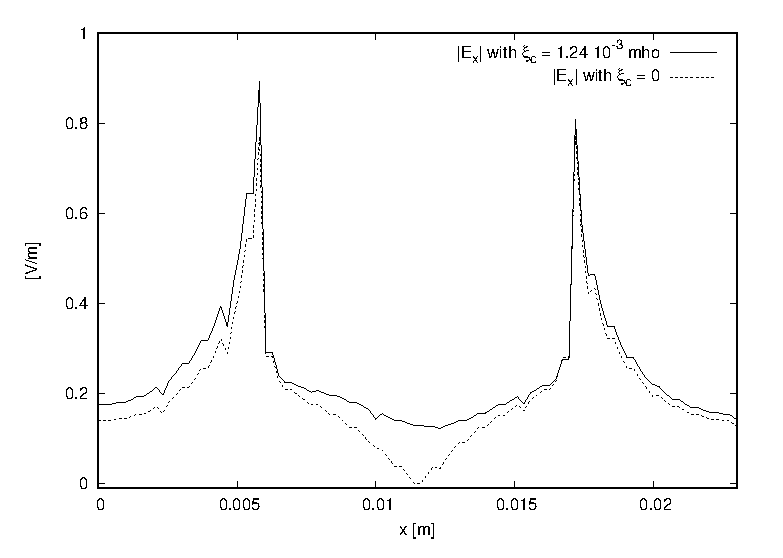
\includegraphics[width=\textwidth]{figure_wu_jaggard_along_x_mag_ex.eps}
\end{subfigure}
%
\begin{subfigure}[b]{0.49\textwidth}
\centering
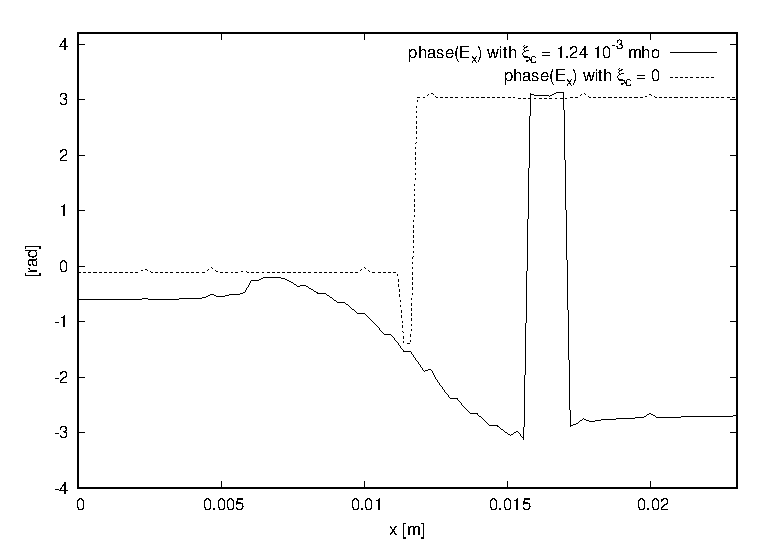
\includegraphics[width=\textwidth]{figure_wu_jaggard_along_x_phase_ex.eps}
\end{subfigure}
\caption{The magnitude and phase of the $x$ component of electric field along a line parallel to $x$ axis 
and passing though the center of gravity of the domain for problem involving 
medium in \cite{wujaggard}. 
The plot for bianisotropic case  using $\xi_c = 1.24\,10^{-3}$ mho is compared with 
the solution obtained in isotropic case using $\xi_c = 0$.}
\label{fi:wu_jaggard_xaxis_ex}
\end{figure}

\begin{figure}
\centering
\begin{subfigure}[b]{0.49\textwidth}
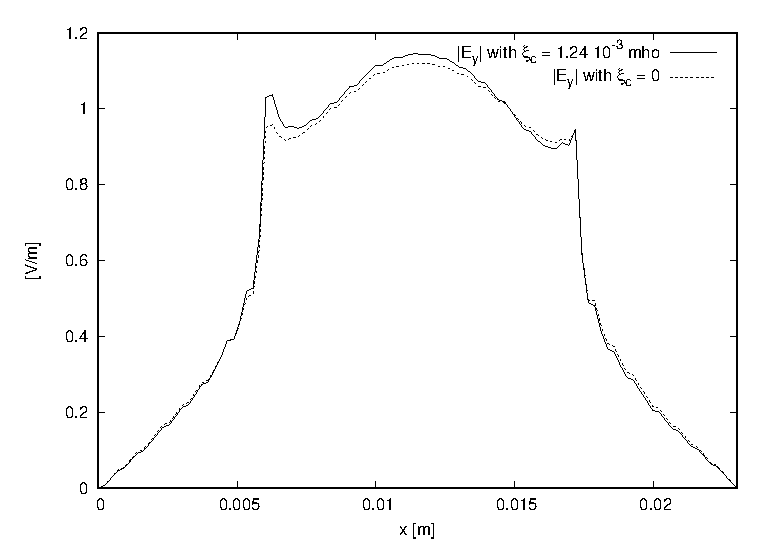
\includegraphics[width=\textwidth]{figure_wu_jaggard_along_x_mag_ey.eps}
\end{subfigure}
%
\begin{subfigure}[b]{0.49\textwidth}
\centering
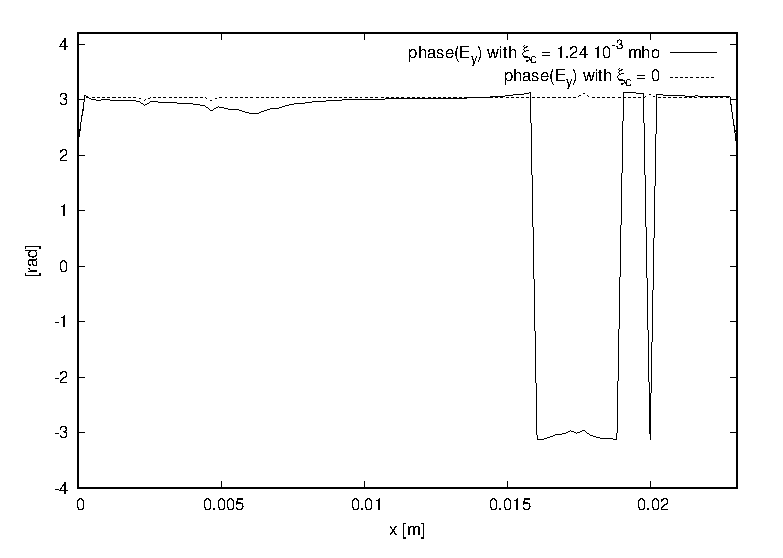
\includegraphics[width=\textwidth]{figure_wu_jaggard_along_x_phase_ey.eps}
\end{subfigure}
\caption{The magnitude and phase of the $y$ component of electric field along a line parallel to $x$ axis 
and passing though the center of gravity of the domain for problem involving 
medium in \cite{wujaggard}. 
The plot for bianisotropic case  using $\xi_c = 1.24\,10^{-3}$ mho is compared with 
the solution obtained in isotropic case using $\xi_c = 0$.}
\label{fi:wu_jaggard_xaxis_ey}
\end{figure}

\begin{figure}
\centering
\begin{subfigure}[b]{0.49\textwidth}
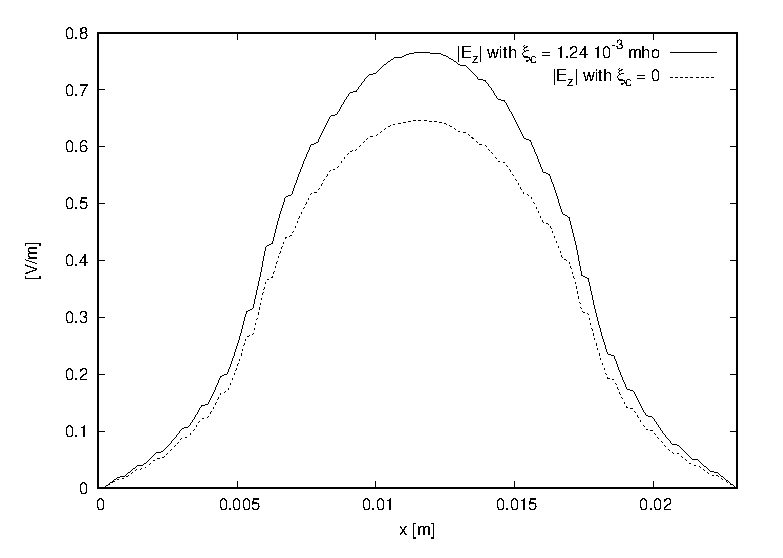
\includegraphics[width=\textwidth]{figure_wu_jaggard_along_x_mag_ez.eps}
\end{subfigure}
%
\begin{subfigure}[b]{0.49\textwidth}
\centering
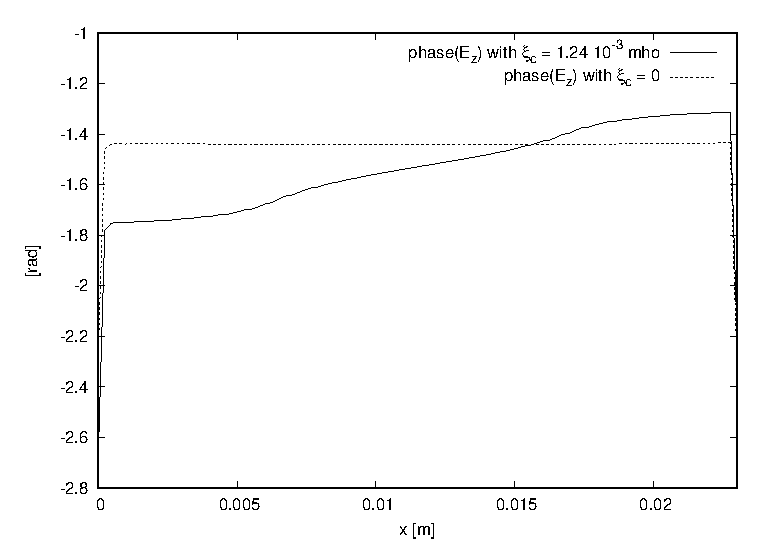
\includegraphics[width=\textwidth]{figure_wu_jaggard_along_x_phase_ez.eps}
\end{subfigure}
\caption{The magnitude and phase of the $z$ component of electric field along a line parallel to $x$ axis 
and passing though the center of gravity of the domain for problem involving 
medium in \cite{wujaggard}. 
The plot for bianisotropic case  using $\xi_c = 1.24\,10^{-3}$ mho is compared with 
the solution obtained in isotropic case using $\xi_c = 0$.}
\label{fi:wu_jaggard_xaxis_ez}
\end{figure}

Similar results are shown in Figures \ref{fi:wu_jaggard_yaxis_ex} to 
\ref{fi:wu_jaggard_zaxis_ez} for the components of fields along y and 
z directions. 
The bianisotropic effect cause a difference of more than 30 percent of the incident 
field  as can be seen from Figure  \ref{fi:wu_jaggard_yaxis_ex}.

\begin{figure}
\centering
\begin{subfigure}[b]{0.49\textwidth}
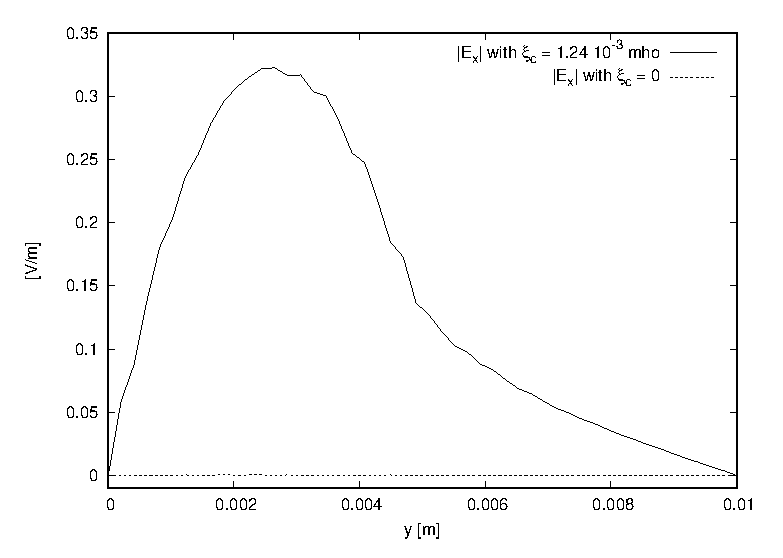
\includegraphics[width=\textwidth]{figure_wu_jaggard_along_y_mag_ex.eps}
\end{subfigure}
%
\begin{subfigure}[b]{0.49\textwidth}
\centering
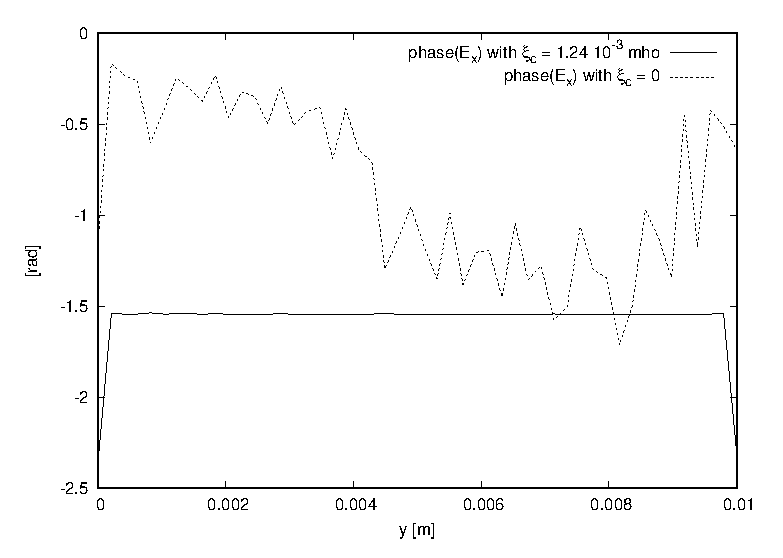
\includegraphics[width=\textwidth]{figure_wu_jaggard_along_y_phase_ex.eps}
\end{subfigure}
\caption{The magnitude and phase of the $x$ component of electric field along a line parallel to $y$ axis 
and passing though the center of gravity of the domain for problem involving 
medium in \cite{wujaggard}. 
The plot for bianisotropic case  using $\xi_c = 1.24\,10^{-3}$ mho is compared with 
the solution obtained in isotropic case using $\xi_c = 0$.}
\label{fi:wu_jaggard_yaxis_ex}
\end{figure}

\begin{figure}
\centering
\begin{subfigure}[b]{0.49\textwidth}
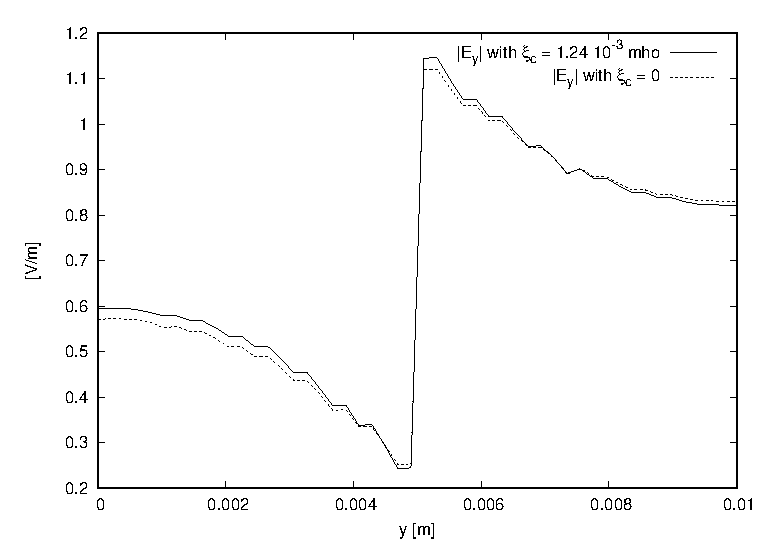
\includegraphics[width=\textwidth]{figure_wu_jaggard_along_y_mag_ey.eps}
\end{subfigure}
%
\begin{subfigure}[b]{0.49\textwidth}
\centering
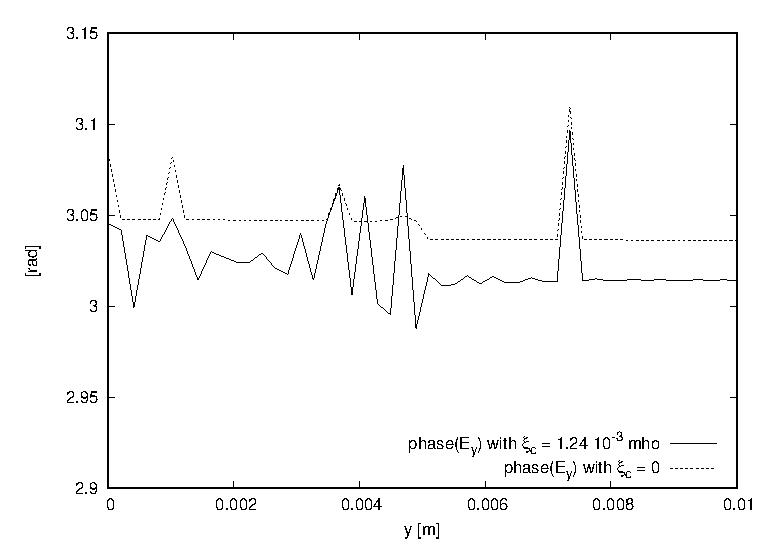
\includegraphics[width=\textwidth]{figure_wu_jaggard_along_y_phase_ey.eps}
\end{subfigure}
\caption{The magnitude and phase of the $y$ component of electric field along a line parallel to $y$ axis 
and passing though the center of gravity of the domain for problem involving 
medium in \cite{wujaggard}. 
The plot for bianisotropic case  using $\xi_c = 1.24\,10^{-3}$ mho is compared with 
the solution obtained in isotropic case using $\xi_c = 0$.}
\label{fi:wu_jaggard_yaxis_ey}
\end{figure}

\begin{figure}
\centering
\begin{subfigure}[b]{0.49\textwidth}
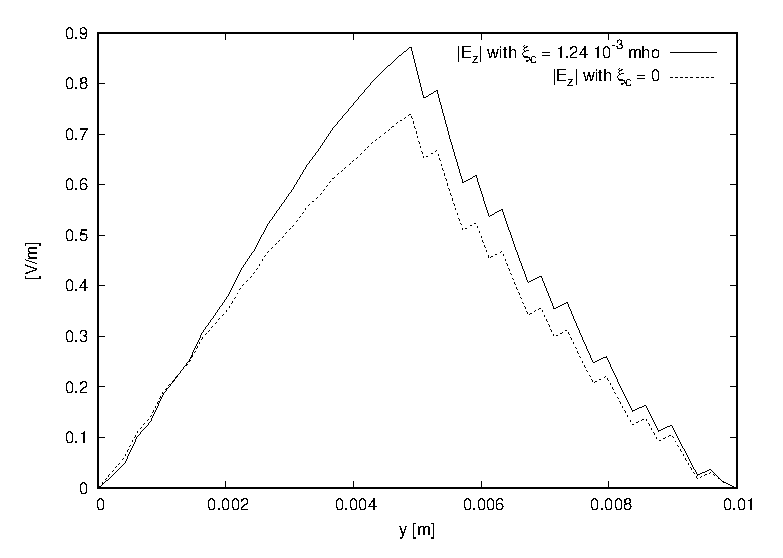
\includegraphics[width=\textwidth]{figure_wu_jaggard_along_y_mag_ez.eps}
\end{subfigure}
%
\begin{subfigure}[b]{0.49\textwidth}
\centering
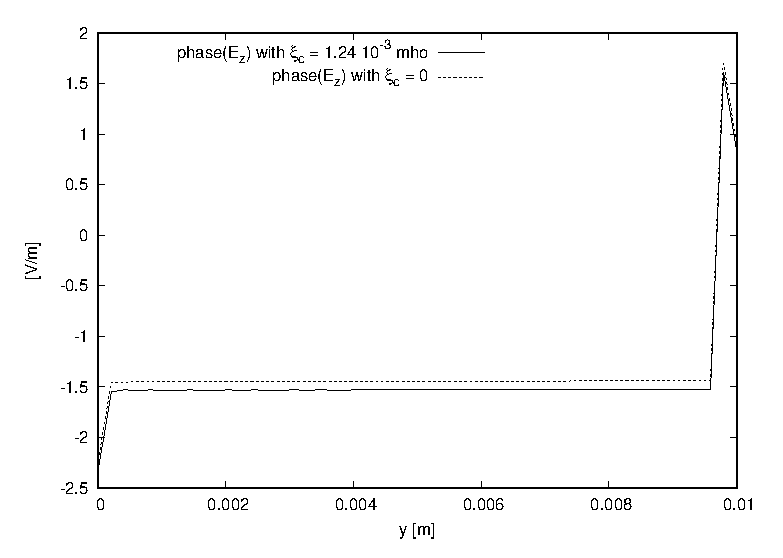
\includegraphics[width=\textwidth]{figure_wu_jaggard_along_y_phase_ez.eps}
\end{subfigure}
\caption{The magnitude and phase of the $z$ component of electric field along a line parallel to $y$ axis 
and passing though the center of gravity of the domain for problem involving 
medium in \cite{wujaggard}. 
The plot for bianisotropic case  using $\xi_c = 1.24\,10^{-3}$ mho is compared with 
the solution obtained in isotropic case using $\xi_c = 0$.}
\label{fi:wu_jaggard_yaxis_ez}
\end{figure}

\begin{figure}
\centering
\begin{subfigure}[b]{0.49\textwidth}
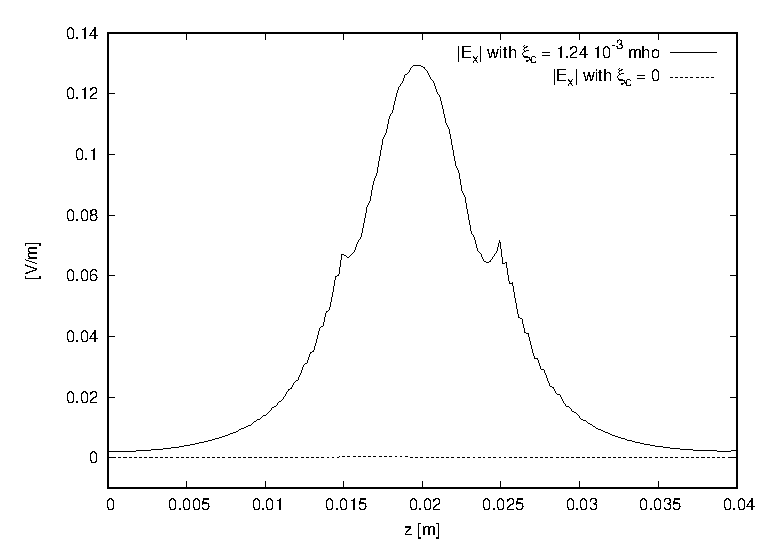
\includegraphics[width=\textwidth]{figure_wu_jaggard_along_z_mag_ex.eps}
\end{subfigure}
%
\begin{subfigure}[b]{0.49\textwidth}
\centering
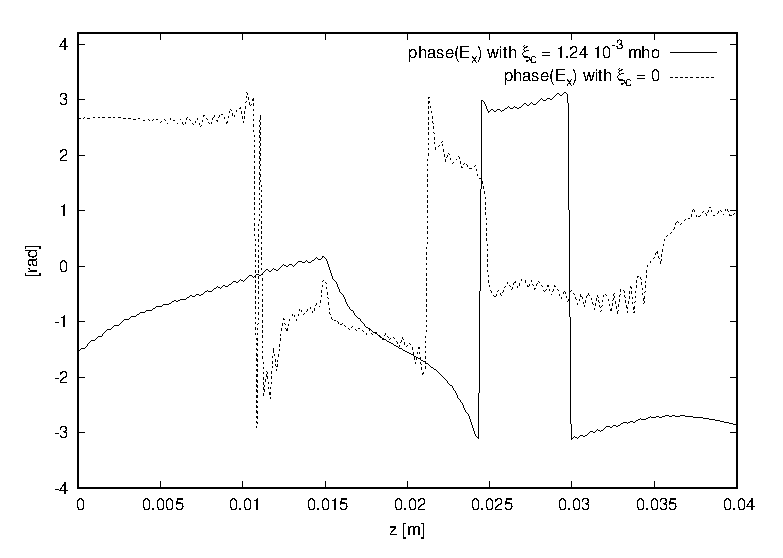
\includegraphics[width=\textwidth]{figure_wu_jaggard_along_z_phase_ex.eps}
\end{subfigure}
\caption{The magnitude and phase of the $x$ component of electric field along a line parallel to $z$ axis 
and passing though the center of gravity of the domain for problem involving 
medium in \cite{wujaggard}. 
The plot for bianisotropic case  using $\xi_c = 1.24\,10^{-3}$ mho is compared with 
the solution obtained in isotropic case using $\xi_c = 0$.}
\label{fi:wu_jaggard_zaxis_ex}
\end{figure}

\begin{figure}
\centering
\begin{subfigure}[b]{0.49\textwidth}
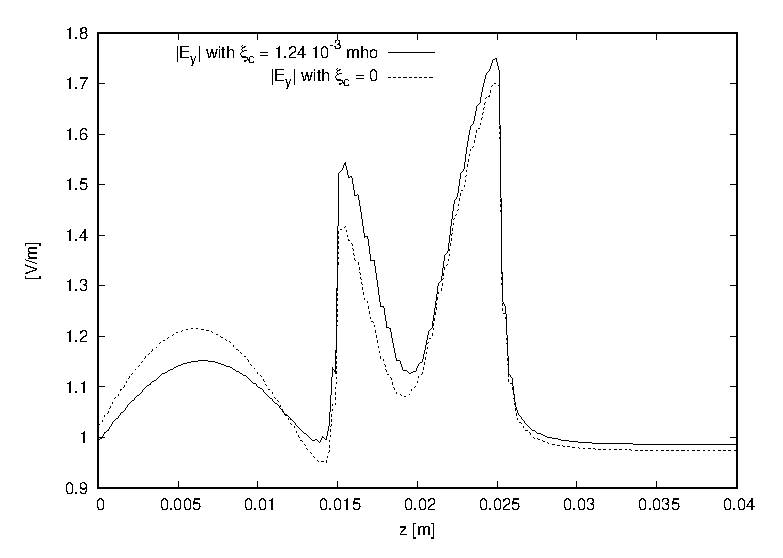
\includegraphics[width=\textwidth]{figure_wu_jaggard_along_z_mag_ey.eps}
\end{subfigure}
%
\begin{subfigure}[b]{0.49\textwidth}
\centering
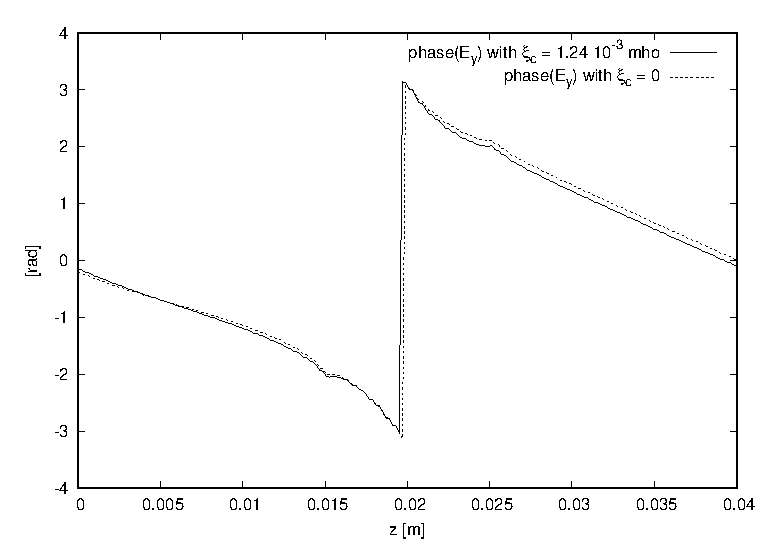
\includegraphics[width=\textwidth]{figure_wu_jaggard_along_z_phase_ey.eps}
\end{subfigure}
\caption{The magnitude and phase of the $y$ component of electric field along a line parallel to $z$ axis 
and passing though the center of gravity of the domain for problem involving 
medium in \cite{wujaggard}. 
The plot for bianisotropic case  using $\xi_c = 1.24\,10^{-3}$ mho is compared with 
the solution obtained in isotropic case using $\xi_c = 0$.}
\label{fi:wu_jaggard_zaxis_ey}
\end{figure}

\begin{figure}
\centering
\begin{subfigure}[b]{0.49\textwidth}
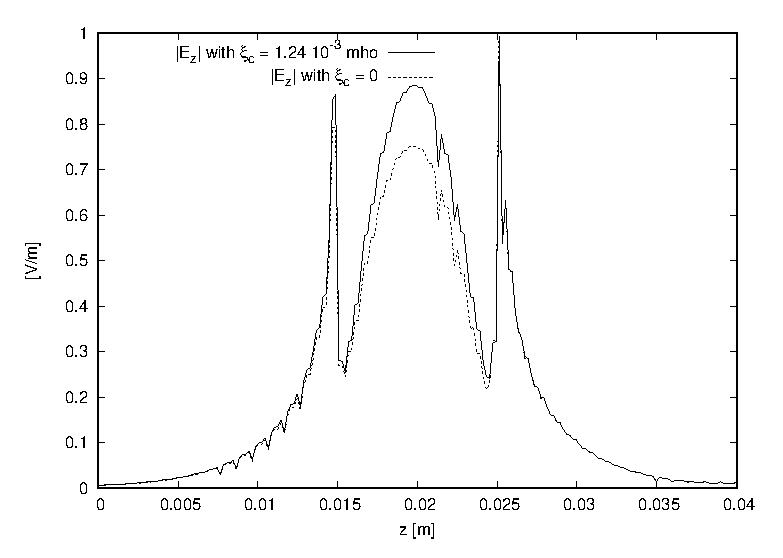
\includegraphics[width=\textwidth]{figure_wu_jaggard_along_z_mag_ez.eps}
\end{subfigure}
%
\begin{subfigure}[b]{0.49\textwidth}
\centering
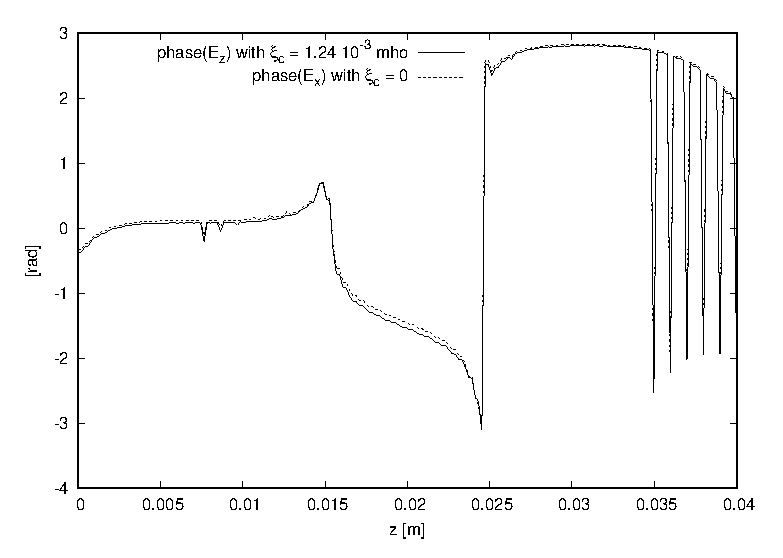
\includegraphics[width=\textwidth]{figure_wu_jaggard_along_z_phase_ez.eps}
\end{subfigure}
\caption{The magnitude and phase of the $z$ component of electric field along a line parallel to $z$ axis 
and passing though the center of gravity of the domain for problem involving 
medium in \cite{wujaggard}. 
The plot for bianisotropic case  using $\xi_c = 1.24\,10^{-3}$ mho is compared with 
the solution obtained in isotropic case using $\xi_c = 0$.}
\label{fi:wu_jaggard_zaxis_ez}
\end{figure}

As mentioned earlier, together, these results provide a bench mark for other approaches 
to solving such problems, owing to the reliability of the results provided here which
is guaranteed by the recently developed theory.
The previous theory \cite{bianisotropi_m3as} was not able to manage these problems and 
our results are therefore novel.
The significant bianisotropic effects demonstrated in the results show the practical
importance of the theory for such media.
